\documentclass[11pt]{article}
\usepackage[margin=0.75in]{geometry}
\usepackage{graphicx}
\usepackage{amsmath}
\usepackage{hyperref}
\usepackage{enumitem}
\usepackage{tikz}
\usepackage{xcolor}
\usetikzlibrary{shapes,arrows,positioning,fit,backgrounds}

\title{\textbf{Solstice: Technical Architecture}}
\author{Computer Vision + Multi-LLM Pipeline for Medical Document Verification}
\date{}

\begin{document}
\maketitle

\section{Executive Summary}

Solstice verifies medical claims against source documents using computer vision and orchestrated LLM processing. The system extracts structured content from PDFs through Detectron2, then runs claims through a multi-stage LLM pipeline that includes evidence extraction, verification, visual analysis, and completeness checking with automatic re-verification when new evidence is found.

\section{Core Architecture}

\subsection{System Design}

Three decoupled layers handle document processing:

\begin{verbatim}
+-------------+          +---------------+          +-------------+
|   Gateway   |  <---->  | Fact Checker  |  <---->  |  Ingestion  |
+-------------+          +---------------+          +-------------+
\end{verbatim}

The Gateway accepts document uploads and claim submissions from users, returning job IDs for async processing. When a document arrives, the Ingestion layer runs first to process the PDF and extract structured JSON. Once ingestion completes, the Fact Checker orchestrates a multi-stage verification pipeline: Evidence Extractor finds relevant quotes, Evidence Verifier validates accuracy, Visual Analyzer processes figures/tables, and Completeness Checker ensures nothing is missed. If new evidence surfaces, a second verification pass runs. Users poll the Gateway for results, which retrieves the consolidated evidence report.

\subsection{Document Processing Pipeline}

\textbf{Layout Detection:}
\begin{itemize}
\item Detectron2 with ResNet-50 identifies document regions
\item 400 DPI rendering for accurate text extraction
\item Bounding box post-processing resolves overlaps
\item Outputs structured JSON with spatial coordinates
\end{itemize}

\begin{figure}[htbp]
\centering
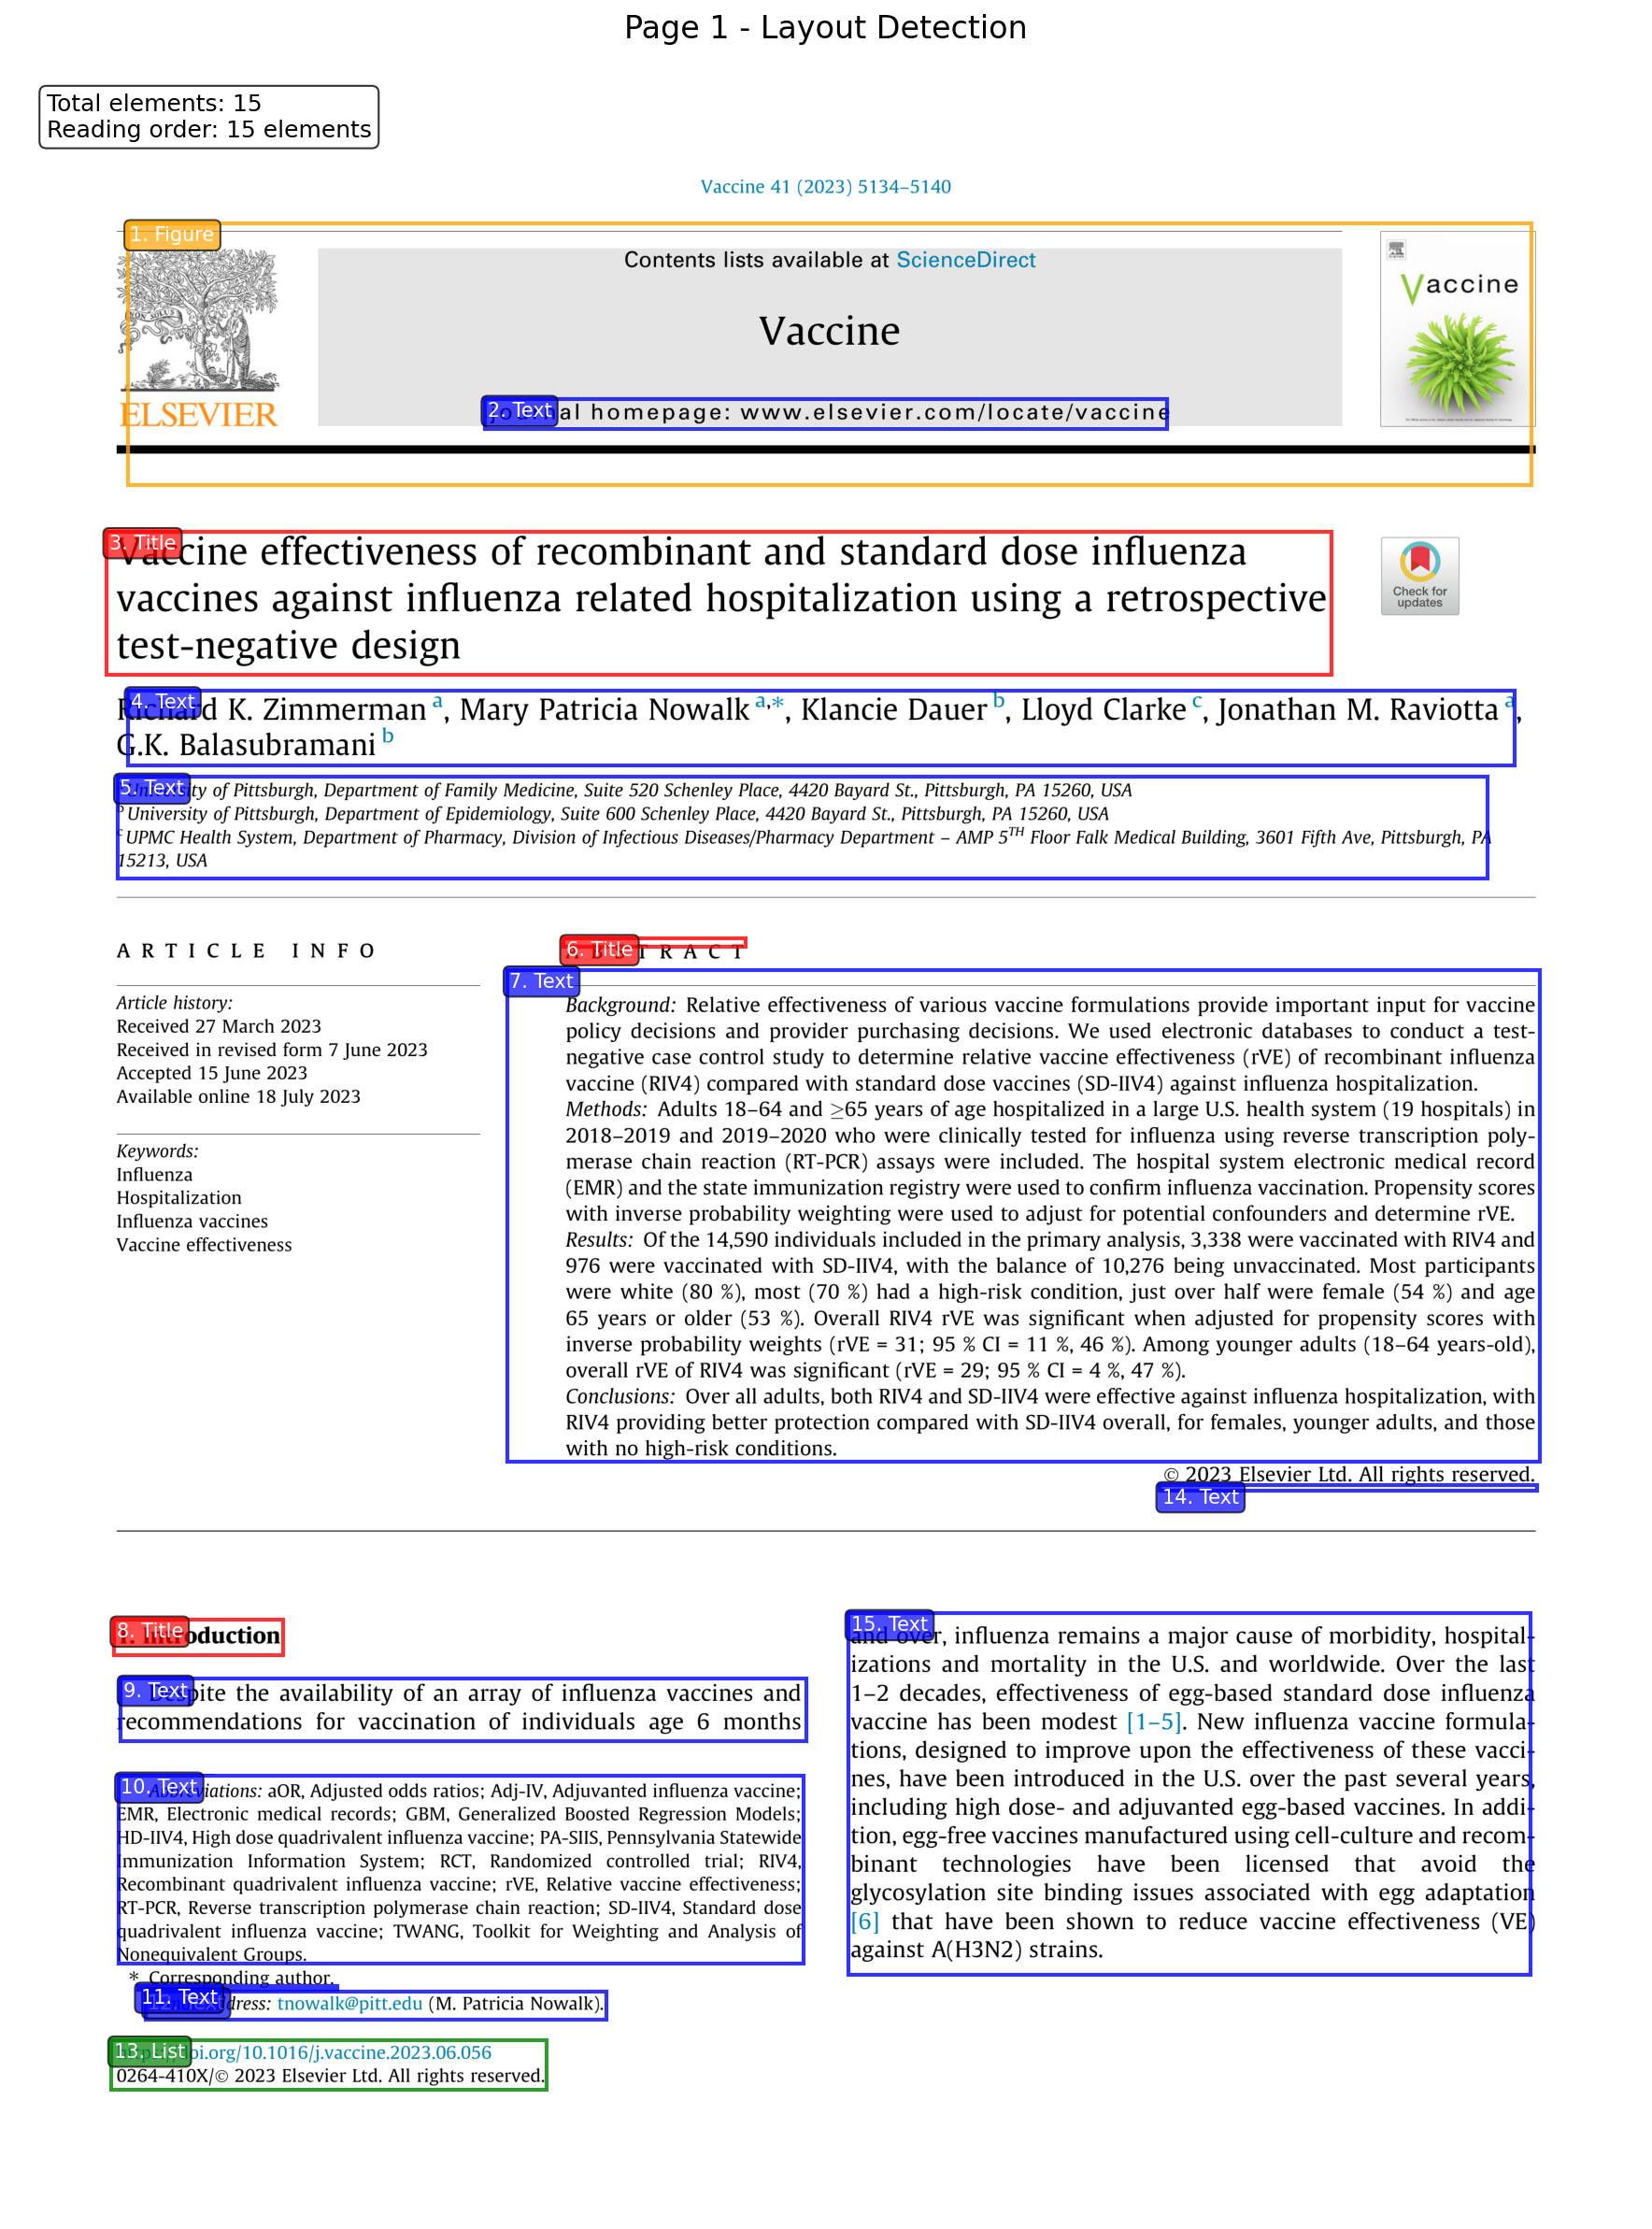
\includegraphics[width=0.85\textwidth]{scientific_layout_example.png}
\caption{Detectron2 identifies text blocks, tables, and figures in medical documents.}
\end{figure}

\section{Claim Verification Pipeline}

\subsection{Multi-Stage LLM Processing}

Claims pass through five specialized LLM components in sequence:

\newpage
\begin{verbatim}
                        Text Pipeline
+-----------------+     +------------------+     +-------------------+
|                 |     |                  |     |                   |
| Claim + Document|---->| Evidence        |---->| Completeness      |
|                 |     | Extractor (LLM) |     | Checker (LLM)     |
+-----------------+     +------------------+     +-------------------+
                                                           |
                                                           v
                                                 +-------------------+
                                                 |                   |
                                                 | Evidence Verifier |
                                                 | V2 (LLM)          |
                                                 +-------------------+
                                                           |
                        Image Pipeline                     |
+-----------------+     +------------------+               |
|                 |     |                  |               |
| Images + Claim  |---->| Visual Analyzer  |---------------+
|                 |     | (Multimodal LLM) |               |
+-----------------+     +------------------+               v
                                                 +-------------------+
                                                 |                   |
                                                 | Evidence Presenter|
                                                 | (LLM)             |
                                                 +-------------------+
\end{verbatim}

\subsection{LLM Components}

\textbf{Evidence Extractor}
\begin{itemize}
\item Finds quotes supporting the claim
\item Returns JSON with evidence and relevance scores
\end{itemize}

\textbf{Evidence Verifier}
\begin{itemize}
\item Validates quote accuracy against source
\item Checks for cherry-picking and missing context
\end{itemize}

\textbf{Completeness Checker}
\begin{itemize}
\item Runs after initial extraction to find additional evidence
\item Ensures all relevant quotes are captured before verification
\end{itemize}

\textbf{Visual Analyzer}
\begin{itemize}
\item Processes tables/figures using multimodal LLM
\item Runs in parallel after text pipeline completes
\end{itemize}

\textbf{Evidence Presenter}
\begin{itemize}
\item Consolidates all verified evidence from text and images
\item Generates final evidence report for users
\end{itemize}

\section{Implementation Patterns}

\subsection{Orchestration}

ClaimOrchestrator manages the verification workflow:
\begin{itemize}
\item Async LLM calls with configurable timeouts
\item Exponential backoff for rate limit handling
\item State transitions through extraction, verification, and completion
\end{itemize}

\subsection{Caching Strategy}

Filesystem cache enables debugging and reprocessing:

\begin{verbatim}
data/cache/{document_name}/
    extracted/
        content.json      # Structured document content
        figures/          # Extracted images
    agents/               # LLM outputs
        claims/
            claim_{id}/
                evidence_extractor/output.json
                evidence_verifier/output.json
                completeness_checker/output.json
                image_evidence_analyzer/{figure_id}/output.json
\end{verbatim}

\section{Scaling Considerations}

\textbf{Ingestion}: CPU-bound on Detectron2, benefits from GPU acceleration

\textbf{Fact Checking}: I/O bound on LLM APIs, scales with concurrent claims

\textbf{Gateway}: Stateless handlers scale horizontally

\section{Marketing Document Adaptation}

Marketing materials use adjusted parameters:
\begin{itemize}
\item Lower confidence threshold (0.1 vs 0.2)
\item Enhanced overlap resolution for creative layouts
\item Same LLM prompts maintain consistency
\end{itemize}

\begin{figure}[htbp]
\centering
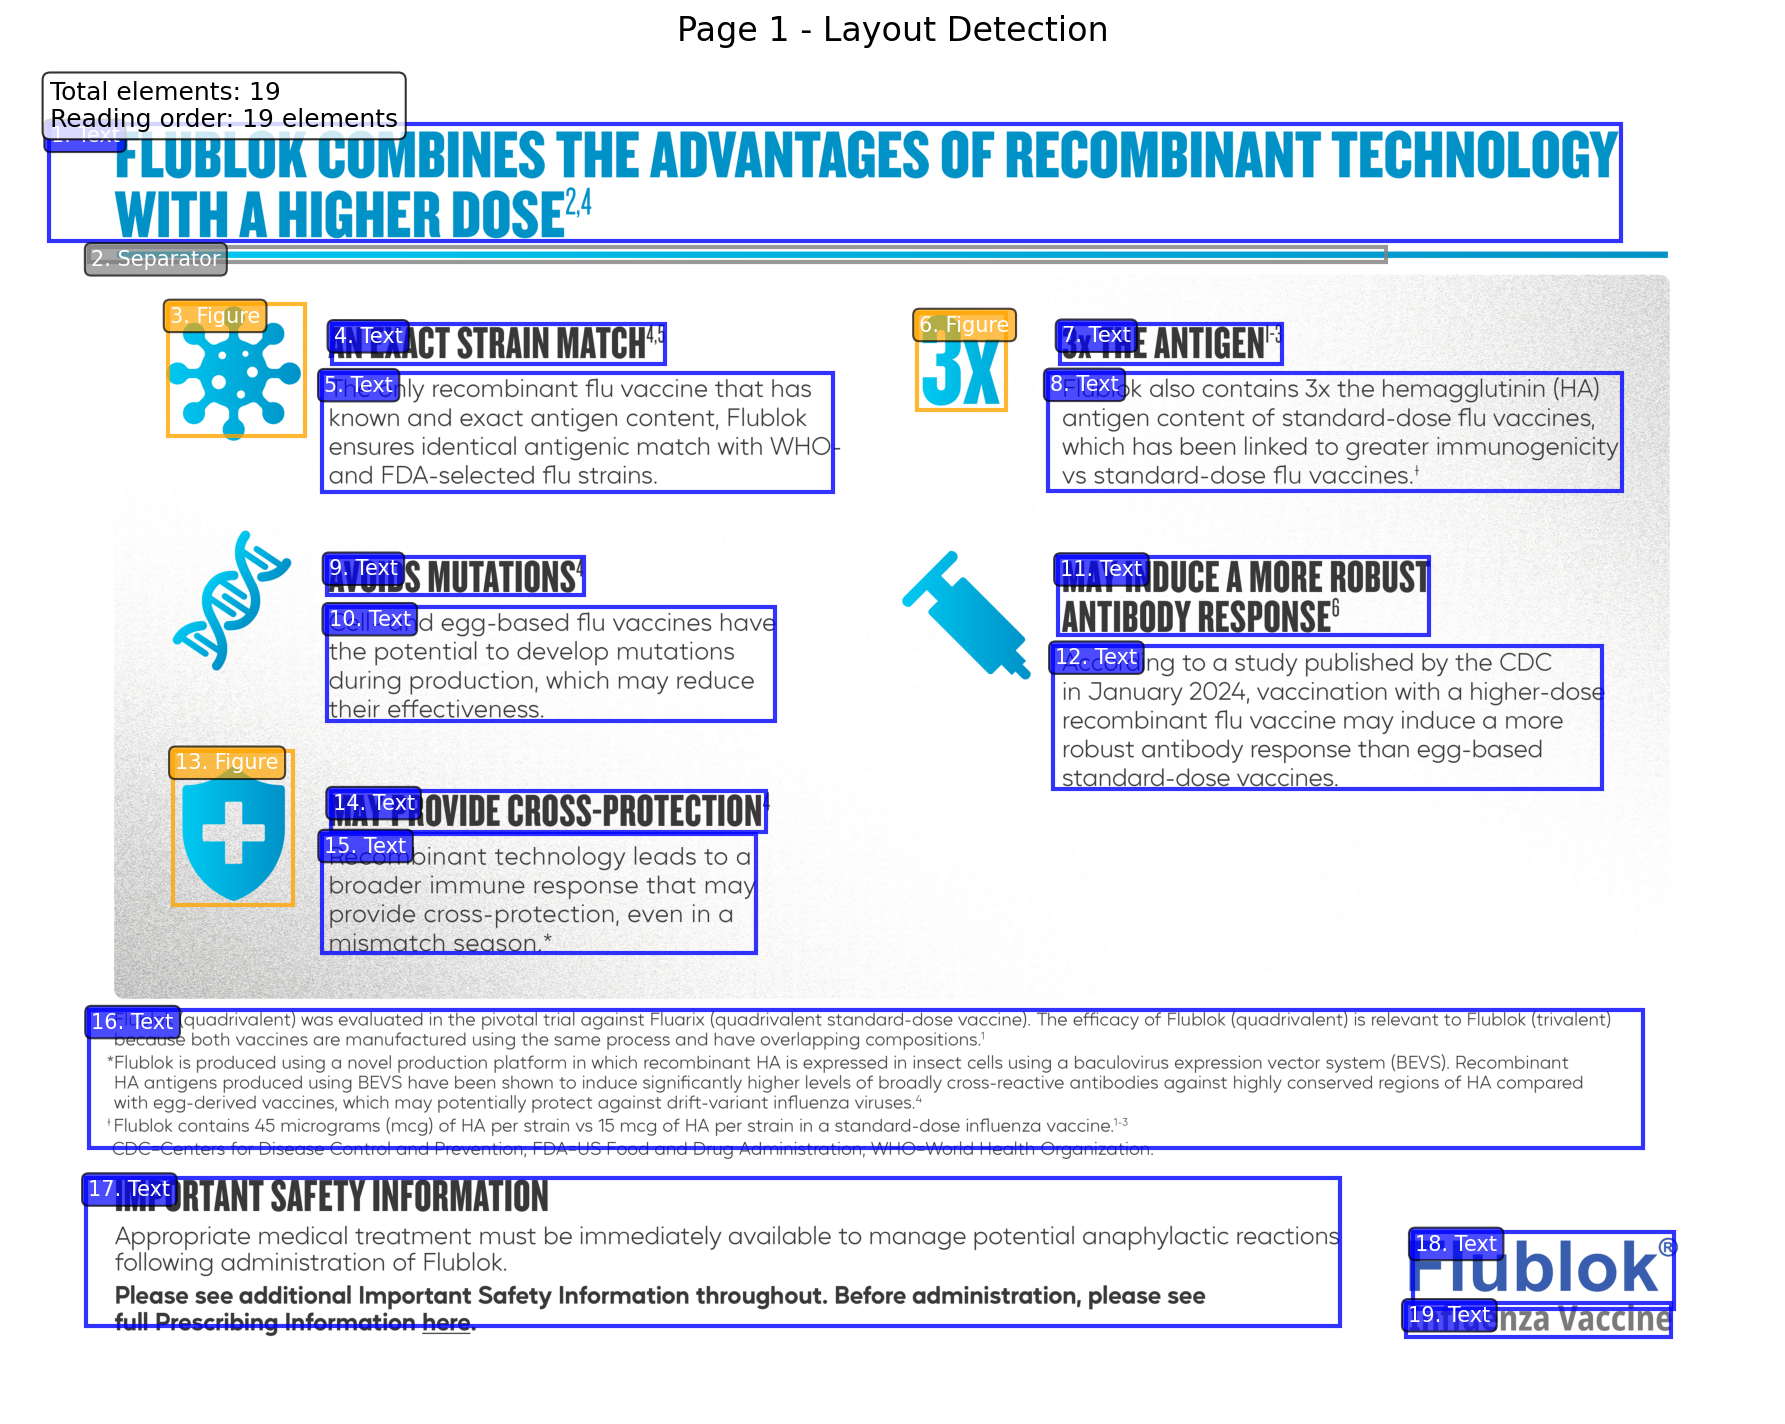
\includegraphics[width=0.85\textwidth]{marketing_layout_example.png}
\caption{Marketing documents require lower confidence thresholds for design-heavy layouts.}
\end{figure}

\end{document}